\documentclass[../../main]{subfiles}

\renewcommand\thesection{\arabic{section}}


\begin{document}

\section{Thermal Control and Exhaust System} \label{sec:thermalControlAndExhaustSystem}

\subsection{Heating / Cooling Element}

The \emph{thermals} of the Incubator can be controlled using a \emph{peltier} module, which is
\emph{semi-conductor} based \emph{heat engine}. The COP\footnote{Coefficient of Performance.} is
much less than a typical \emph{compressor} based \emph{heat engines} and is \emph{variable} depending
on the current passing through it. But the compactness of the \emph{peltier} cooler makes it preferable
to this design. One another disadvantage to this type of cooling is that it requires a proper \emph{exhaust}
system. The \emph{peltier} cooler only decrease the temperature of its \emph{cold} side to relative to its
\emph{hot} side\footnote{The \emph{cold} side will be $30 - 40^\circ$C colder than its \emph{hot} side.}.
The \emph{peltier} module is thin, that means the \emph{hot} and \emph{cold} are closer. So it is
\emph{crucial} to properly pull away the heat from its \emph{cold} side as fast as possible.

We will be using \emph{TEC12703} peltier, which has the specification of:

\begin{itemize}
    \item \textbf{Operating voltage.:} $3\si{V}$ to $15\si{V}$.
    \item \textbf{I Max.:} $3\si{A}$.
    \item \textbf{Power:} $30\si{W}$.
\end{itemize}

Figures \ref{fig:peltierImage} and \ref{fig:peltierHSImage} shows the peltier and the heatsink
used.

\begin{center}
    {\begin{minipage} [c] {0.45\textwidth}
        \centering
        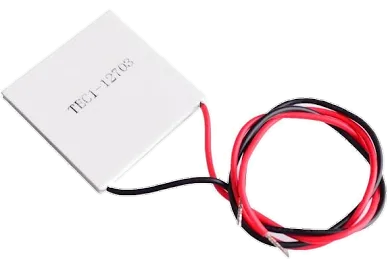
\includegraphics [
            max width = \IGXMaxWidth,
            max height = \IGXMaxHeight,
            \IGXDefaultOptionalArgs,
        ] {pics/peltier.png}
        \captionof{figure} {
            \emph{TEC12703} peltier module.
            \label{fig:peltierImage}
        }
    \end{minipage}
    \hfill
    \begin{minipage} [c] {0.45\textwidth}
        \centering
        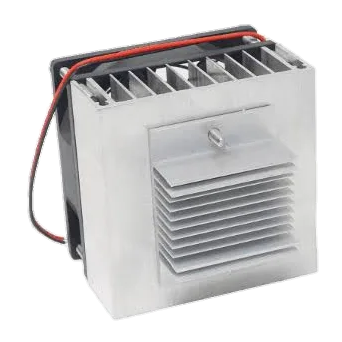
\includegraphics [
            max width = \IGXMaxWidth,
            max height = \IGXMaxHeight,
            \IGXDefaultOptionalArgs,
        ] {pics/peltier_hs.png}
        \captionof{figure} {
            Heat sink for \emph{TEC12703} peltier module.
            \label{fig:peltierHSImage}
        }
    \end{minipage}\hfill}
\end{center}

\subsection{Three Chambered Exhaust}

\begin{center}
    {\begin{minipage} [c] {0.55\textwidth}
        So we can make a three chambered exhaust system to heat or cool our incubator. We can
        make the cooling side of the peltier into an chamber likewise the heating side into
        another chamber. And we will have another common chamber that is always connected to the
        incubator. By using panels we can connect the desired chamber with the common chamber.
        Thereby, cooling or heating the incubator. We would need almost 7 panels to accomplish this
        task. And we can use relays to control these panels. Figure \ref{fig:relControl} shows a
        relay controlling circuit.

        We can choose the bjt as \emph{BC547}, diode as \emph{1N4007} and base resistance as
        $4.7\si{k \ohm}$.

    \end{minipage}
    \hfill
    \begin{minipage} [c] {0.35\textwidth}
        \centering
        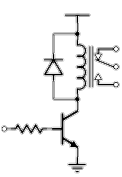
\includegraphics [
            max width = \IGXMaxWidth,
            max height = \IGXMaxHeight,
            \IGXDefaultOptionalArgs,
        ] {pics/relctrl.png}
        \captionof{figure} {
            Relay controlling circuit.
            \label{fig:relControl}
        }
    \end{minipage}\hfill}
\end{center}

\begin{center}
    {\begin{minipage} [c] {0.55\textwidth}

        Figure \ref{fig:relaySugarCubeImage} shows the relay sugar cube we are
        using.

        Specification:

        \begin{itemize}
            \item \textbf{Operating voltage:} $12\si{V}$.
            \item \textbf{Operating current:} $70\si{mA}$.
        \end{itemize}

    \end{minipage}
    \hfill
    \begin{minipage} [c] {0.35\textwidth}
        \centering
        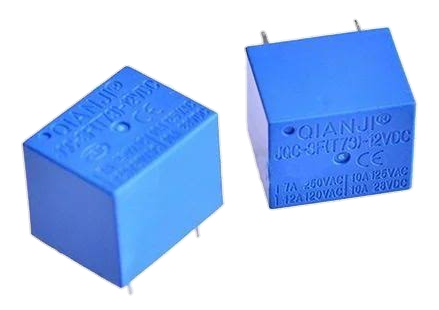
\includegraphics [
            max width = \IGXMaxWidth,
            max height = \IGXMaxHeight,
            \IGXDefaultOptionalArgs,
        ] {pics/sugar_cube.png}
        \captionof{figure} {
            Relay sugar cubes.
            \label{fig:relaySugarCubeImage}
        }
    \end{minipage}\hfill}
\end{center}

There will be two relays that controls the direction of panels. Each of these will
have their NC connected to ground, and NO connected to 5V. We will use the 7th bit
of the $16$ bit shift register to control these relays. One relay will be connected
directly\footnote{the base of the \emph{BC547} in the controlling circuit} to the 7th
bit and the other is connected an inverter in between.

And we will arrange the 7 relays that controls the panel in parallel between the common
pins of these two \emph{direction relays}. $0^{\mbox{th}}$ to $6^{\mbox{th}}$ bits will trigger
each of these relays.

The $12^{\mbox{th}}$ bit will control the peltier and the fan connected to it.

\alertNote{
    Peltier module is also controlled via a relay, since it can pull almost $2.7A$ when
    connected to a 12V power supply.
}

\subsection{Air Flow Controlling}

\begin{center}
    {\begin{minipage} [c] {0.55\textwidth}
        The air of the exhaust is controlled using three fans, one is directly connected to the
        peltier and the other two connected to the $13^{\mbox{th}}$ and $14^{\mbox{th}}$ bits
        of the shift register. Figure \ref{fig:fanImage} show that 12V fan we are using.

        Specification:

        \begin{itemize}
            \item \textbf{Operating voltage:} $12\si{V}$.
            \item \textbf{Operating current:} $220\si{mA}$.
        \end{itemize}

    \end{minipage}
    \hfill
    \begin{minipage} [c] {0.35\textwidth}
        \centering
        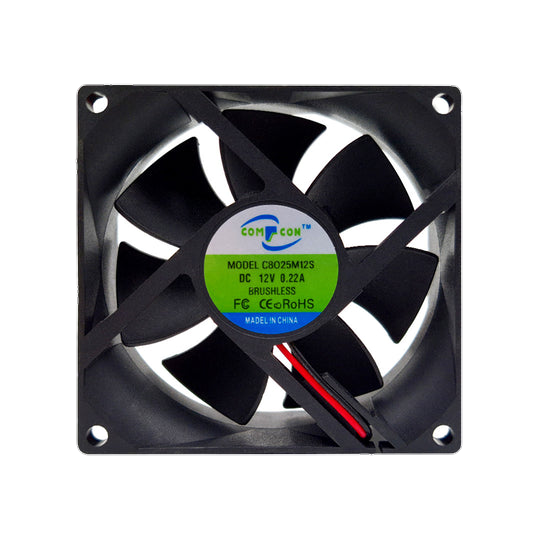
\includegraphics [
            max width = \IGXMaxWidth,
            max height = \IGXMaxHeight,
            \IGXDefaultOptionalArgs,
        ] {pics/fan.png}
        \captionof{figure} {
            12V DC brushless fan.
            \label{fig:fanImage}
        }
    \end{minipage}\hfill}
\end{center}

\begin{center}
    {\begin{minipage} [c] {0.55\textwidth}
        Inorder to low side switch the fans, we need to
        use a power transistor, as the fans can pull 220mA.
        We have chosen \emph{CD148D}, as the switching transistor.
        And the \emph{BC547} is used to drive this power transistor.
        Refer figure \ref{fig:fanControl} for more information about
        the circuit.

    \end{minipage}
    \hfill
    \begin{minipage} [c] {0.35\textwidth}
        \centering
        \includegraphics [
            max width = \IGXMaxWidth,
            max height = \IGXMaxHeight,
            \IGXDefaultOptionalArgs,
        ] {tikzpics/endFanControl.pdf}
        \captionof{figure} {
            Circuit to low side switch the fans.
            \label{fig:fanControl}
        }
    \end{minipage}\hfill}
\end{center}

%\begin{center}
%    {\begin{minipage} [c] {0.45\textwidth}
%        \centering
%        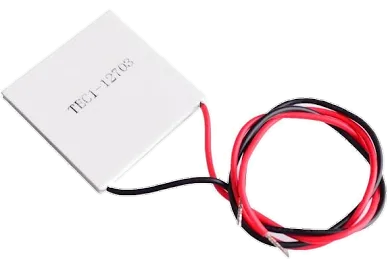
\includegraphics [
%            max width = \IGXMaxWidth,
%            max height = \IGXMaxHeight,
%            \IGXDefaultOptionalArgs,
%        ] {pics/peltier.png}
%        \captionof{figure} {
%            \emph{TEC12703} peltier module.
%            \label{fig:peltierImage}
%        }
%    \end{minipage}
%    \hfill
%    \begin{minipage} [c] {0.45\textwidth}
%        \centering
%        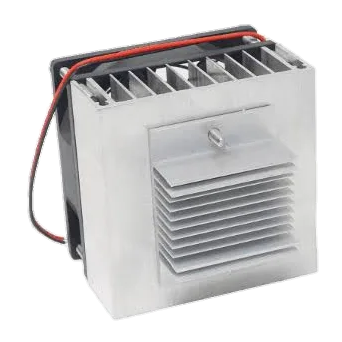
\includegraphics [
%            max width = \IGXMaxWidth,
%            max height = \IGXMaxHeight,
%            \IGXDefaultOptionalArgs,
%        ] {pics/peltier_hs.png}
%        \captionof{figure} {
%            Heat sink for \emph{TEC12703} peltier module.
%            \label{fig:peltierHSImage}
%        }
%    \end{minipage}\hfill}
%\end{center}

%\begin{figure}
%    \centering
%    \includegraphics [
%        max width = \IGXMaxWidth,
%        max height = \IGXMaxHeight,
%        \IGXDefaultOptionalArgs,
%    ] {tikzpics/endAbsDirectionControlModule.pdf}
%    \captionof{figure} {}
%    \label{fig:absPanelActuatorModule}
%\end{figure}

%\begin{figure}
%    \centering
%    \includegraphics [
%        max width = \textwidth,
%        max height = \textheight,
%        \IGXDefaultOptionalArgs,
%    ] {tikzpics/endAbsExhaustPanelControlSystem.pdf}
%    \captionof{figure} {}
%    \label{fig:absExhaustPanelControlSystem}
%\end{figure}

\end{document}
